\documentclass[14pt]{report}
\usepackage[utf8]{inputenc}
\usepackage[russian]{babel}
\usepackage{textcomp}
\usepackage{indentfirst}
\usepackage{graphicx}
\usepackage{alltt}
\usepackage{amsfonts}
\usepackage{amsmath}


\begin{document} 

\section{Задание 1}	
\subsection{Задание 1.1}
Средства просмотра системной информации \\
Цель работы: Изучение команд для получения информации о системе. \\
history\\
\begin{figure}[h!]
\centering
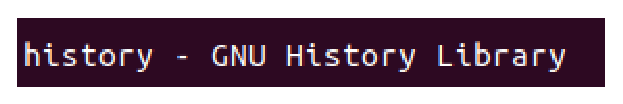
\includegraphics [width=1\textwidth]{mhistory}\\
\end{figure}
nano\\
\begin{figure}[h!]
\centering
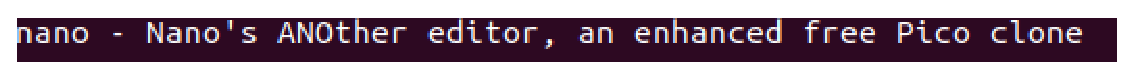
\includegraphics [width=1\textwidth]{mnano}\\
\end{figure}
cd\\
\begin{figure}[h!]
\centering
\includegraphics [width=1\textwidth]{mcd}\\
\end{figure}
cp\\
\begin{figure}[h!]
\centering
\includegraphics [width=1\textwidth]{mcp}\\
\end{figure}
mv\\
\begin{figure}[h!]
\centering
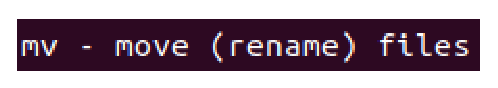
\includegraphics [width=1\textwidth]{mmv}\\
\end{figure}
rm\\
\begin{figure}[h!]
\centering
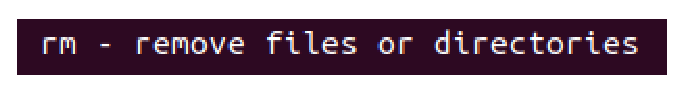
\includegraphics [width=1\textwidth]{mrm}\\
\end{figure}
df\\
\begin{figure}[h!]
\centering
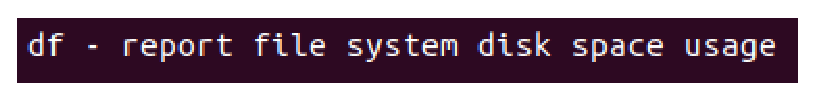
\includegraphics [width=1\textwidth]{mdf}\\
\end{figure}
du\\
\begin{figure}[h!]
\centering
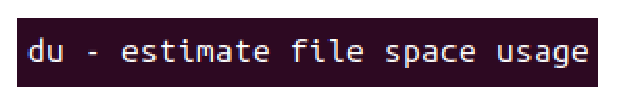
\includegraphics [width=1\textwidth]{mdu}\\
\end{figure}
free\\
\begin{figure}[h!]
\centering
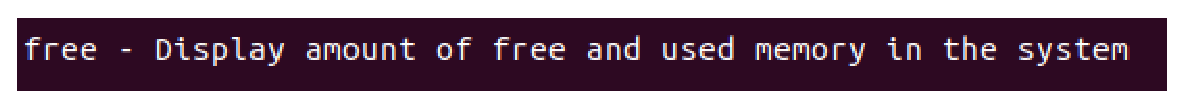
\includegraphics [width=1\textwidth]{mfree}\\
\end{figure}
top\\
\begin{figure}[h!]
\centering
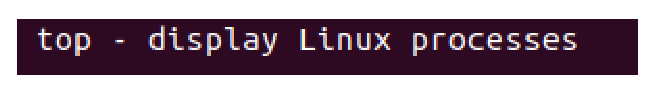
\includegraphics [width=1\textwidth]{mtop}\\
\end{figure}
ls\\
\begin{figure}[h!]
\centering
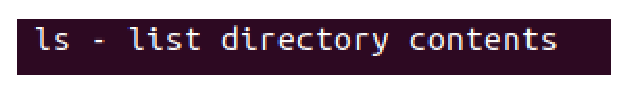
\includegraphics [width=1\textwidth]{mls}\\
\end{figure}
mkdir\\
\begin{figure}[h!]
\centering
\includegraphics [width=1\textwidth]{mmkdir}\\
\end{figure}
pwd\\
\begin{figure}[h!]
\centering
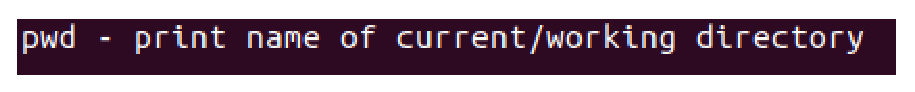
\includegraphics [width=1\textwidth]{mpwd}\\
\end{figure}
clear\\
\begin{figure}[h!]
\centering
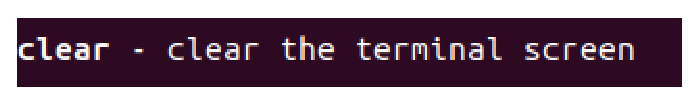
\includegraphics [width=1\textwidth]{mclear}\\
\end{figure}
exit\\
\begin{figure}[h!]
\centering
\includegraphics [width=1\textwidth]{mexit}\\
\end{figure}
uname\\
\begin{figure}[h!]
\centering
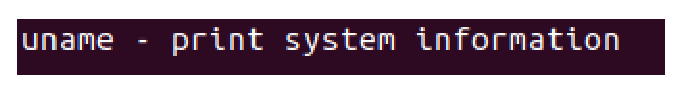
\includegraphics [width=1\textwidth]{muname}\\
\end{figure}
vmstat\\
\begin{figure}[h!]
\centering
\includegraphics [width=1\textwidth]{mvmstat}\\
\end{figure}
man\\
\begin{figure}[h!]
\centering
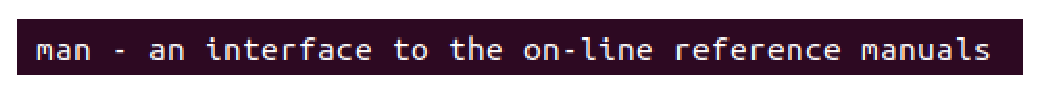
\includegraphics [width=1\textwidth]{mman}\\
\end{figure}
ifconfug\\
\begin{figure}[h!]
\centering
\includegraphics [width=1\textwidth]{mifconfug}\\
\end{figure}
lsmod\\
\begin{figure}[h!]
\centering
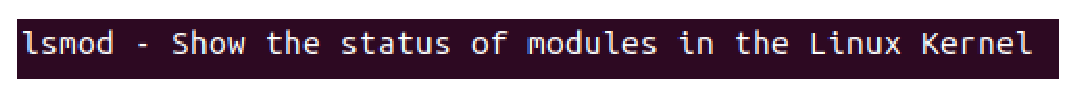
\includegraphics [width=1\textwidth]{mlsmod}\\
\end{figure}
date\\
\begin{figure}[h!]
\centering
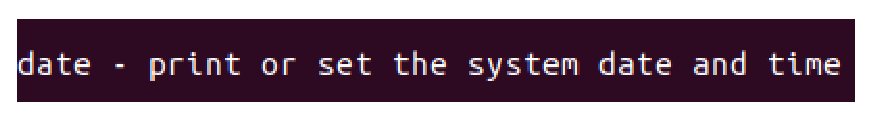
\includegraphics [width=1\textwidth]{mdate}\\
\end{figure}
uptime\\
\begin{figure}[h!]
\centering
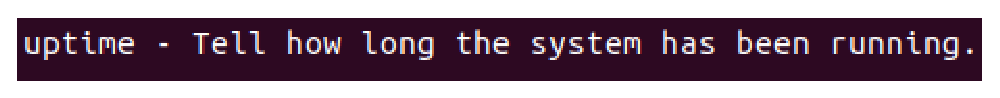
\includegraphics [width=1\textwidth]{muptime}\\
\end{figure}
Задание 1.1(a)\\
Показать нагруженность системы. \\
Была выбрана команда htop, поскольку она выводит больший перечень процессов и обладаем элементами выборочной сортировки.\\
\begin{figure}[h!]
\centering
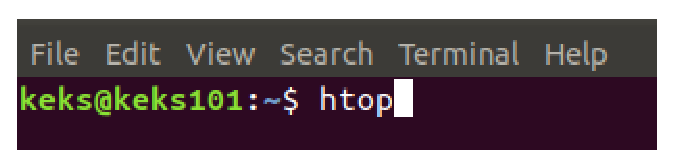
\includegraphics [width=1\textwidth]{htop0}\\
\end{figure}
\begin{figure}[h!]
\centering
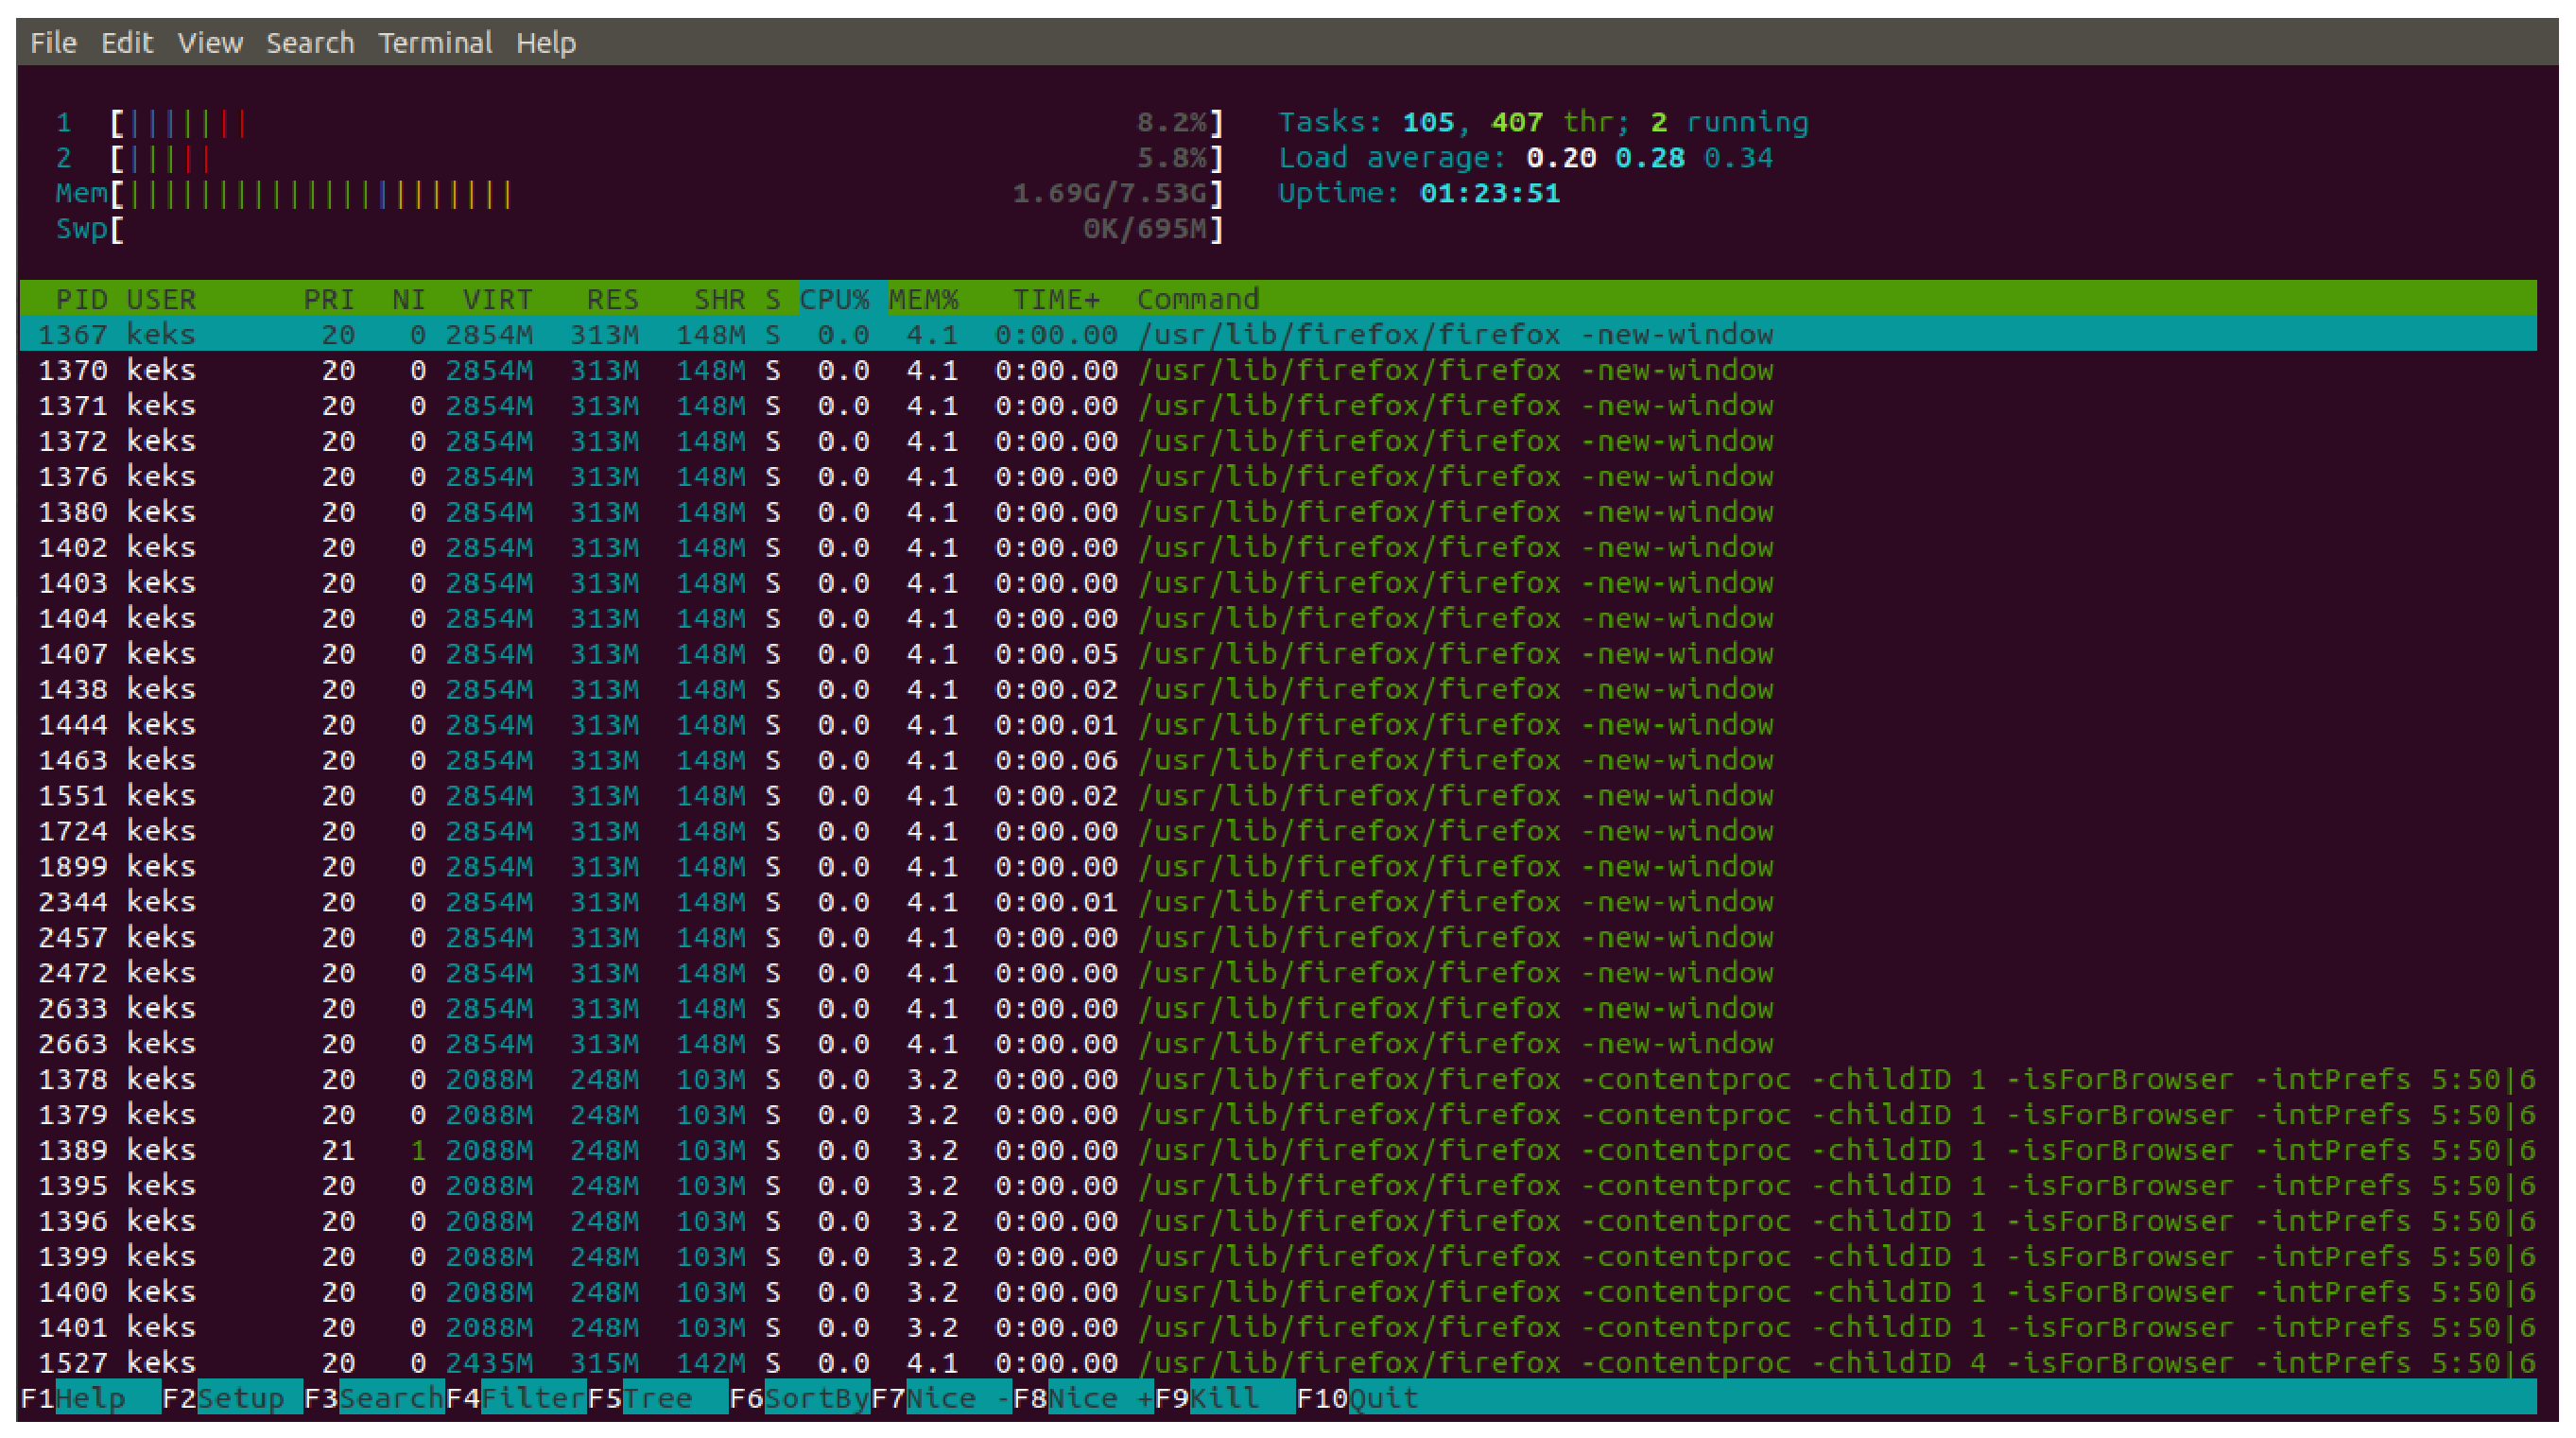
\includegraphics [width=1\textwidth]{htop}\\
\end{figure}

Задание 1.1(b)\\
Отобразить объем занятой оперативной памяти в килобайтах (Кб).\\
Была выбрана команда free соответственно с ключом kilo.\\

\begin{figure}[h!]
\centering
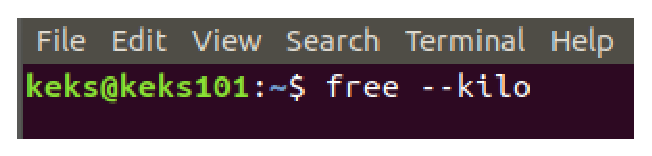
\includegraphics [width=1\textwidth]{free0}\\
\end{figure}
\begin{figure}[h!]
\centering
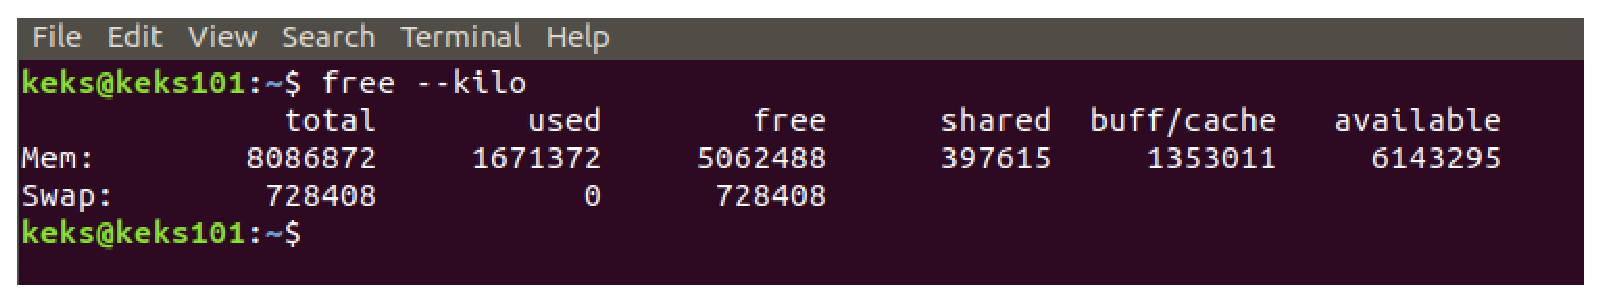
\includegraphics [width=1\textwidth]{free}\\
\end{figure}

\end{document} 